\documentclass[10pt]{beamer}

\usetheme{CUDenver}

\usepackage{mathtools}
\usepackage[abs]{overpic}
\setlength\unitlength{1mm}

\usepackage{color}
\usepackage{graphicx}
\usepackage{url}
\usepackage{xspace}
\usepackage{tikz}
\usetikzlibrary{arrows,positioning}
\usepackage{subfigure}
\usepackage{verbatim}
\usepackage{amsfonts}
\usepackage{amsmath}
\usepackage{amssymb}
\usepackage{amsbsy}
\usepackage{amsthm}
\usepackage[mathcal]{euscript}
\usepackage{algorithmic}
\usepackage{boxedminipage}
\usepackage{fancyvrb}
\usepackage{epstopdf}
\usepackage[lined,ruled]{algorithm2e}

\newcommand{\tred}[1]{\textcolor{Red}{#1}}
\newcommand{\tgreen}[1]{\textcolor{Green}{#1}}
\newcommand{\tcyan}[1]{\textcolor{Cyan}{#1}}
\newcommand{\tyellow}[1]{\textcolor{Yellow}{#1}}
\newcommand{\tpurple}[1]{\textcolor{Purple}{#1}}
\newcommand{\tblack}[1]{\textcolor{Black}{#1}}
\newcommand{\tgrey}[1]{\textcolor{Grey}{#1}}
\newcommand{\tdeepred}[1]{\textcolor{deepred}{#1}}
\definecolor{Green}{rgb}{0,.5,0}
%use for definitions
\definecolor{Red}{rgb}{.8,.2,0}
%use for emphasis
\definecolor{Yellow}{rgb}{.6,.6,.1}
%use for part titles
\definecolor{Cyan}{rgb}{.2,.6,.7}
%use for comments
\definecolor{Purple}{rgb}{.4,0,1}
%use for examples
\definecolor{deepred}{rgb}{.53,.29,.24}
%use for important points
\definecolor{Black}{rgb}{0,0,0}
%use for washout
\definecolor{Grey}{rgb}{.45,.45,.45}
%%%%%%%%%%%%%%%%%%%%%%%%%%%%%%%%%%%%%%%%%%%%%%%%%%%%%%%%%%%%%%%%%%%%%%%%%%%%%%%%
% newcommands.tex

% itemize with the explaining text left justified afer the item
% Example:
%   \itembox{CNR} The Control net reduction
%   \itembox{A} Another item
% renders as
% * CNR   The Control net reduction
% * A     Another item
\newcommand{\itembox}[1]{\item {\makebox[0.80in]{#1 \hfill}}}

% Abbreviations 
\newcommand{\ie}{{\itshape i.e.}}
\newcommand{\eg}{{\itshape e.g.}}

% Bold symbols
\newcommand{\bs}[1]{\boldsymbol{#1}}

% Cardinality
\newcommand{\card}[1]{n\left(#1\right)} %{\left|#1\right|}

% Math Operators
\DeclareMathOperator*{\argmin}{arg\,min}
\DeclareMathOperator*{\argmax}{arg\,max}

% Standard Probability
\DeclareMathOperator{\E}{\mathbb{E}}
\DeclareMathOperator*{\P}{\mathbb{P}}

% Data-Consistent Inversion Framework


% Parameter Space

\DeclareMathOperator*{\param}{\lambda}
\DeclareMathOperator*{\pspace}{\Lambda}
\newcommand{\pmeas}{\mu_{\pspace}}
\newcommand{\pborel}{\mathcal{B}_{\pspace}}

\DeclareMathOperator*{\initialP}{\P_{\text{in}}}
\DeclareMathOperator*{\initial}{\pi_{\text{in}}}
\DeclareMathOperator*{\updatedP}{\P_{\text{up}}}
\DeclareMathOperator*{\updated}{\pi_{\text{up}}}

\DeclareMathOperator*{\data}{\boldsymbol{d}}
\DeclareMathOperator*{\dspace}{\mathcal{D}}
\newcommand{\dmeas}{\mu_{\dspace}}
\newcommand{\dborel}{\mathcal{B}_{\dspace}}

\DeclareMathOperator*{\q}{Q\left (\param \right )}
\DeclareMathOperator*{\M}{\mathcal{M}}

\DeclareMathOperator*{\obsP}{\P_{\text{ob}}}
\DeclareMathOperator*{\obs}{\pi_{\text{ob}}}
\DeclareMathOperator*{\predP}{\P_{\text{pr}}}
\DeclareMathOperator*{\pred}{\pi_{\text{pr}}}




%%%%%%%%%%%%%%%%%%%%%%%%%%%%%%%%%%%%%%%%%%%%%%%%%%%%%%%%%%%%%%%%%%%%%%%%%%%%%%%%

 
\synctex=1
\tikzset{
    %Define standard arrow tip
    >=stealth',
    %Define style for boxes
    punkt/.style={
           rectangle,
           rounded corners,
           draw=black, very thick,
           text width=6.5em,
           minimum height=2em,
           text centered},
    % Define arrow style
    pil/.style={
           ->,
           thick,
           shorten <=2pt,
           shorten >=2pt,}
}

\usepackage[english]{babel}

\newtheorem{assumption}{Assumption}
\newtheorem{defn}{Definition}


\author{Michael Pilosov\\ \vskip 5pt{Advisor: Troy Butler}}%* \vskip 3pt Troy Butler}
\title[CG]{How Geometric Features\\of Quantity of Interest Maps\\Impact Errors and Convergence\\of Sample-Based Solutions\\to Stochastic Inverse Problems}
\institute{University of Colorado Denver}
\date{\today}
\begin{document}


\begin{frame}[t,plain]
    \titlepage
\end{frame}


%%%%%%%%%%%%%%%%%%%%%%%%%%%%%%%%%%%%%%%%%%%%%%%%%%%%%%%%%%%
\section{Notation and Terminology}
% start the content of the presentation
\subsection{Broad Goals of Uncertainty Quantification}
%%%%%%%%%%%%%%%%%%%%%%%%%%%%%%%%%%%%%%%%%%%%%%%%%%%%%%%%%%
\begin{frame}[t]

\begin{itemize}
	\item Quantify and reduce uncertainty
	\vskip 20pt
	\item Be \emph{accurate} and \emph{precise}
	\vskip 20pt
	\item Make inferences and predictions
	\vskip 20pt
	\item Design ``efficient'' experiments
	\vskip 20pt
	\item Collect and use data ``intelligently''
\end{itemize}

\end{frame}

\subsection{Formal Definitions}
%%%%%%%%%%%%%%%%%%%%%%%%%%%%%%%%%%%%%%%%%%%%%%%%%%%%%%%%%%
\begin{frame}[t]
%\vskip 25pt
\centering
\begin{figure}
\centering

\begin{tikzpicture}[node distance=2cm, auto,]
 %nodes
 
 % We make a dummy figure to make everything look nice.
 \node[] (dummy) {};
  \node[right=of dummy] (data) {$\dspace$};
  
  \node[punkt, inner sep=5pt,below=of dummy]
 (model) {Model \\ (PDE)}
 	edge[pil,->, bend right=25] node[right] {$Q(u\lam)$} (data);

 \node[left=of dummy] (pspace) {$\Lambda$}
   edge[pil,->, bend right=45] node[left] {$u\lam$} (model)
   edge[pil,->, bend left=45] node[above] {$Q\lam$} (data);
   
   
\end{tikzpicture}

\vspace{1em}
\emph{Defining the Quantity of Interest Map}
\end{figure}

\end{frame}


%%%%%%%%%%%%%%%%%%%%%%%%%%%%%%%%%%%%%%%%%%%%%%%%%%%%%%%%%%
\begin{frame}{The QoI Map}

\only<1>{

\begin{figure}[h]
	\includegraphics[width=0.85\textwidth]{./figures/threelevels/schematic_lambda_solution_data}
\end{figure}

}

\only<2>{

\begin{figure}[h]
	\includegraphics[width=0.85\textwidth]{./figures/threelevels/schematic_lambda_data}
\end{figure}

}

\only<3>{

\begin{figure}[h]
	\includegraphics[width=0.85\textwidth]{./figures/threelevels/schematic_lambda_data_level1}
\end{figure}

}

\end{frame}

%%%%%%%%%%%%%%%%%%%%%%%%%%%%%%%%%%%%%%%%%%%%%%%%%%%%%%%%%%
\begin{frame}{A Forward UQ Problem}

\begin{figure}[h]
	\includegraphics[width=0.85\textwidth]{./figures/threelevels/schematic_lambda_data_level3}
\end{figure}

{We denote the measurable spaces of parameters and data on the QoI as $(\pspace,\pborel)$ and $(\dspace,\dborel)$, respectively.}
\bigskip

\tdeepred{Given some prior density $\pri$ on $(\pspace,\pborel)$, we let $\pfpr$ denote the push-forward of this density on $(\dspace,\dborel)$.}

\end{frame}

%%%%%%%%%%%%%%%%%%%%%%%%%%%%%%%%%%%%%%%%%%%%%%%%%%%%%%%%%%
\begin{frame}{The Inverse QoI Map}

\begin{figure}[h]
	\includegraphics[width=0.85\textwidth]{./figures/threelevels/schematic_data_lambda_level1}
\end{figure}

\end{frame}

%%%%%%%%%%%%%%%%%%%%%%%%%%%%%%%%%%%%%%%%%%%%%%%%%%%%%%%%%%
\begin{frame}{An Inverse UQ Problem}

\begin{figure}[h]
	\includegraphics[width=0.85\textwidth]{./figures/threelevels/schematic_data_lambda_level3}
\end{figure}

\tdeepred{Given $\obs$ on $(\dspace,\dborel)$, we let $\pos$ denote the pullback (consistent) density on $(\pspace,\pborel)$.}

\end{frame}


\subsection{Basic Assumptions \& Terminology}
%%%%%%%%%%%%%%%%%%%%%%%%%%%%%%%%%%%%%%%%%%%%%%%%%%%%%%%%%%
\begin{frame}[t]

\begin{itemize}[<+->]
	\item State variable: $u$ {\color{gray}(e.g. heat, energy, pressure, deflection)}
	\vskip 10pt
	\item<.-> Parameters: $\lambda$ {\color{gray}(e.g. source term, diffusion, boundary data)}
	\vskip 10pt
		\item Deterministic model: $\MMM (u, \lambda) = 0$, $$\MMM:\lambda \to u(\lambda)$$

	\item Quantity of Interest map \tdeepred{(QoI)} - at least pcw differentiable \vskip 5pt
		\begin{itemize}[<+->]
		\item Functional of the solution $$q: u(\lambda) \to \RR$$
		\item Can be vector valued $$Q = \mat{c}{q_1\\ q_2\\ \vdots \\ q_d}$$
		\item<.-> $Q(\lambda) := Q(u(\lambda))$
	\end{itemize}
	
\end{itemize}

\end{frame}


\subsection{The Stochastic Inverse Problem}
%%%%%%%%%%%%%%%%%%%%%%%%%%%%%%%%%%%%%%%%%%%%%%%%%%%%%%%%%%
\begin{frame}[t]

\begin{figure}
\centering
	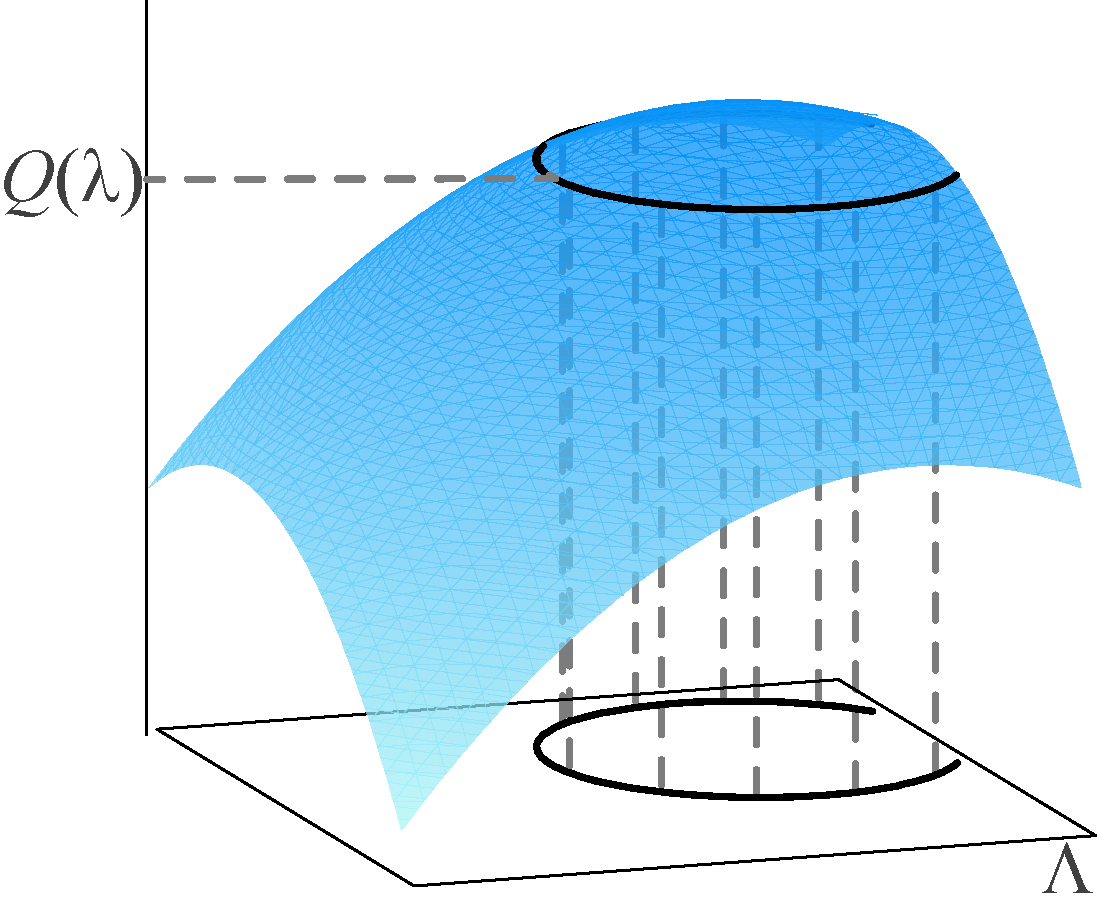
\includegraphics[width=.65\textwidth]{images/illustration1}<1>
	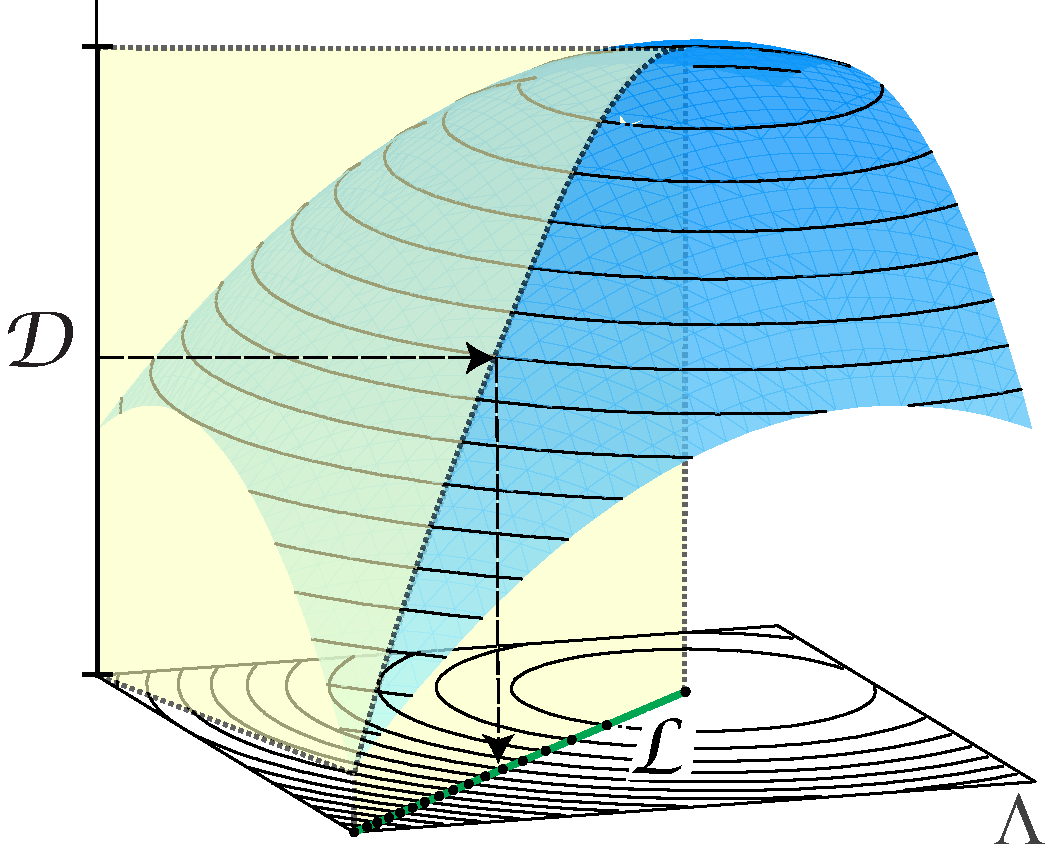
\includegraphics[width=.65\textwidth]{images/illustration2}<2>
	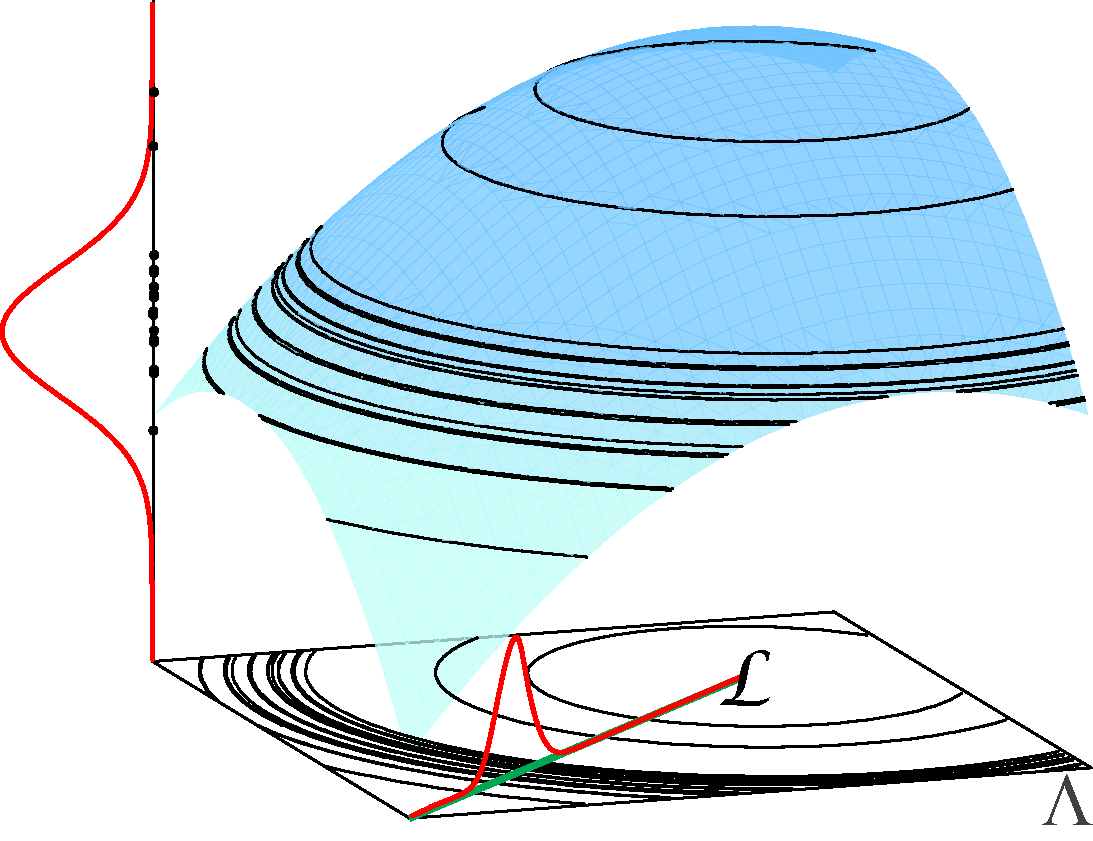
\includegraphics[width=.7\textwidth]{images/illustration3}<3>
\end{figure}
\begin{center}
{\scriptsize Figure adopted from \cite{BET14+} and used with permission}
\end{center}
\end{frame}

%%%%%%%%%%%%%%%%%%%%%%%%%%%%%%%%%%%%%%%%%%%%%%%%%%%%%%%%%%
\begin{frame}[t]

\begin{figure}
\centering
	\includegraphics[width=1\textwidth]{images/troy_mt3contour}
\end{figure}
\begin{center}

{\scriptsize Figure adopted from \cite{BET14+} and used with permission}

\tdeepred{Key Question:} Distinguish (assign probability to) events that belong to same contour. 
\end{center}
\end{frame}

\subsection{Problem Formulation and Solution}
%%%%%%%%%%%%%%%%%%%%%%%%%%%%%%%%%%%%%%%%%%%%%%%%%%%%%%%%%%%
\begin{frame}[t]

\begin{defn}[Inverse Problem]\label{defn:consistency}
Given $\observedP$ on $(\dspace, \dborel)$ the \textbf{inverse problem} is to determine a probability measure $\updatedP$ on $(\pspace, \pborel)$ such that 

	\begin{equation}\label{eq:inv}
		\updatedP(Q^{-1}(E)) = \observedP(E),
	\end{equation}
for all events $E \in \mathcal{B}_\dspace$, where

	\begin{equation*}
		\updated = \frac{d\updatedP}{d\mu_\pspace} \;\text{ and }\; \observed = \frac{d\observedP}{d\mu_\dspace}.
	\end{equation*}
\eqref{eq:inv} defines a \tdeepred{``Consistent Solution,''} yields a \tdeepred{Consistency Condition.}
\end{defn}

Note: {\scriptsize We use the notation $\PP$ and $\pi$ throughout this work to relate measures to their associated densities (i.e., Radon-Nikodym derivatives), which exist under the assumption of a dominating (Lebesgue) volume measure $\mu$.}
\end{frame}


%%%%%%%%%%%%%%%%%%%%%%%%%%%%%%%%%%%%%%%%%%%%%%%%%%%%%%%%%%
\begin{frame}[t]{Perspectives}
\begin{itemize}
	\item We seek the $\updatedP$ whose push-forward measure matches $\observedP$
	\item In measure-theoretic terms, $\updatedP$ is a pull-back measure of $\observedP$

	\begin{defn}[Observed Density]\label{defn:obsden}
		The density $\observed$ in \eqref{eq:inv} represents the uncertainty in QoI data.
	\end{defn}

	\begin{defn}[Initial Density]\label{defn:initialden}
		$\initial$ encodes prior beliefs about $\param$'s (before evidence is accounted for)
	\end{defn}

\end{itemize}

\end{frame}

%%%%%%%%%%%%%%%%%%%%%%%%%%%%%%%%%%%%%%%%%%%%%%%%%%%%%%%%%%
\begin{frame}[t]{Summarizing}
\begin{itemize}
	\item ``Push-forward'' \textbf{initial} beliefs using $\qoi$ to \textbf{compare} to \textbf{observed} (data)
	\item Solve forward problem to construct solution to inverse problem
	\item The push-forward density of $\initial$ under the map $\qoi$ is denoted by $\predicted$

	\begin{defn}[Predicted Density]\label{defn:predicted}
		$\predicted$ is given as the Radon-Nikodym derivative (with respect to $\mu_\dspace$) of the push-forward probability measure defined by:
		\begin{equation}\label{eq:pred}
			\predictedP (E)  = \initialP \left ( \qoi^{-1}(E) \right ), \; \forall \; E \in \dborel.
		\end{equation}
	\end{defn}

\end{itemize}

\end{frame}

%%%%%%%%%%%%%%%%%%%%%%%%%%%%%%%%%%%%%%%%%%%%%%%%%%%%%%%%%%
\begin{frame}[t]
These definitions are combined to form the \textbf{posterior density}, originally derived in \cite{BJW18}:
\begin{equation}\label{eq:post}
\predicted \lam = \initial \lam \frac{\pi_\dspace \q }{\predicted \q }, \; \lambda \in \pspace.
\end{equation}

\begin{itemize}
	\item $\obs$ and $\predicted$ defined on $(\dspace, \dborel)$ are evaluated at $\qlam$
	\item The map $Q$ impacts the structure of the posterior
	\item $\dspace$ itself depends on $Q$
	\item Primary work in solving for $\predicted$ (in \eqref{eq:inv}) requires constructing $\predicted$
	\item This is because $\initial$ and $\obs$ are given \emph{a priori} (often parametric)
	\item Posterior derived through use of Disintegration Theorem in \cite{BJW18}
	\item Existence and Uniqueness provided that we satisfy assumptions
\end{itemize}
\end{frame}



\subsection{Properties and Assumptions of the Posterior}
%%%%%%%%%%%%%%%%%%%%%%%%%%%%%%%%%%%%%%%%%%%%%%%%%%%%%%%%%%
\begin{frame}[t]
\begin{assumption}[Predictability Assumption]\label{as:pred}
The measure associated with $\obs$ is absolutely continuous with respect to the measure associated with $\obs$.
\end{assumption}


The requirement is guaranteed if the following is satisfied:
\begin{equation}\label{eq:pred}
\exists \; C>0 \text{ such that } \obs (d) \leq C \predicted(d) \text{ for a.e. } d\in \dspace,
\end{equation}
where it is understood that $d = Q\lam$ for some $\lambda \in \pspace$.
Assuming \eqref{eq:pred} holds, we restate the following theorem from \cite{BJW18}:
\begin{theorem}[Existence and Uniqueness]
For any set $A\in \pborel$, the solution $\predictedP$ given defined by
\begin{equation}\label{eq:cb_sol}
\predictedP (A) = \int_\dspace \left (  \int_{\pspace \in Q^{-1}(d)}  \initial\lam \frac{\obs\q}{\predicted\q} \, d\mu_{\pspace, d} \lam \right ) \, d\mu_\dspace(d), \; \forall \; A \in \pborel
\end{equation}
is a consistent solution, and is unique up to choice of $P_\pspace$ on $(\pspace, \pborel)$.
\end{theorem}

\end{frame}

%%%%%%%%%%%%%%%%%%%%%%%%%%%%%%%%%%%%%%%%%%%%%%%%%%%%%%%%%%
\begin{frame}[t]

This posterior density \eqref{eq:post} appearing within the iterated integral in \eqref{eq:cb_sol} has no normalization constant (it already integrates to one), which is summarized in Corollary 3.1 in \cite{BJW18} and restated in simplified form below:
\begin{corollary}\label{cor:int}
$\predictedP(\pspace) = 1$.
\end{corollary}

\end{frame}




%%%%%%%%%%%%%%%%%%%%%%%%%%%%%%%%%%%%%%%%%%%%%%%%%%%%%%%%%%
\begin{frame}[t]{Stability}

\begin{defn}{Total Variation / Statistical Distance}
	\begin{equation}\label{eq:tv}
		d_{\text{TV}} (P_f, P_g) := \int \abs{f - g} \, d\mu,
	\end{equation}
\end{defn}
where $f,g$ are the densities (Radon-Nikodym derivatives with respect to $\mu$) associated with measures $P_f, P_g$, respectively.

All the stability results herein are presented with respect to this metric.
\end{frame}

%%%%%%%%%%%%%%%%%%%%%%%%%%%%%%%%%%%%%%%%%%%%%%%%%%%%%%%%%%
\begin{frame}[t]

\begin{defn}[Stability of Posteriors I]\label{defn:stableobs}
Given $\initialP$ and $\observedP$, let $\widehat{\observedP}$ be any perturbation to $\observedP$ on $(\dspace, \dborel)$ satisfying \eqref{eq:pred}.
Let $\predictedP$ and $\widehat{\predictedP}$ denote the consistent solutions associated with $\observedP$ and $\widehat{\observedP}$, respectively.
We say that $\predictedP$ is \emph{stable} with respect to perturbations in $\observedP$ if for all $\eps > 0$, there exists a $\delta > 0$ such that
\begin{equation}
d_{\text{TV}} (\observedP, \widehat{\observedP}) < \delta \implies d_{\text{TV}} (\predictedP, \widehat{\predictedP}) < \eps.
\end{equation}
\end{defn}

In \cite{BJW18}, it is shown that $d_{\text{TV}} (\widehat{\predictedP}, \predictedP) = d_{\text{TV}} (\widehat{\observedP}, \observedP)$, which immediately proves the following:

\begin{theorem}
$\predictedP$ is stable with respect to perturbations in $\observedP$.
\end{theorem}

\end{frame}

%%%%%%%%%%%%%%%%%%%%%%%%%%%%%%%%%%%%%%%%%%%%%%%%%%%%%%%%%%
\begin{frame}[t]
\begin{defn}[Stability of Posteriors II]\label{defn:stableprior}
Given $\initialP$ and $\observedP$, let $\widehat{\initialP}$ be any perturbation to $\initialP$ on $(\pspace, \pborel)$ satisfying \eqref{eq:pred}.
Let $\predictedP$ and $\widehat{\predictedP}$ denote the consistent solutions associated with $\observedP$ and $\widehat{\observedP}$, respectively.
Let $\sett{P_{\pspace, d}}{d\in\dspace}{}$ and $\sett{\widehat{P_{\pspace, d}}}{d\in\dspace}{}$ be the conditional probabilities defined by the disintegration of $\initialP$ and $\widehat{\initialP}$, respectively.
We say that $\predictedP$ is \emph{stable} with respect to perturbations in $\initialP$ if for all $\eps > 0$, there exists a $\delta > 0$ such that for almost every $d\in\supp(\obs)$,
\begin{equation}\label{eq:stableprior}
d_{\text{TV}} (P_{\pspace, d}, \widehat{P_{\pspace, d}}) < \delta \implies d_{\text{TV}} (\predictedP, \widehat{\predictedP}) < \eps.
\end{equation}
\end{defn}

\begin{theorem}
$\predictedP$ is stable with respect to perturbations in the prior.
\label{thm:stableprior}
\end{theorem}


\end{frame}

%%%%%%%%%%%%%%%%%%%%%%%%%%%%%%%%%%%%%%%%%%%%%%%%%%%%%%%%%%
\begin{frame}[t]
\begin{itemize}

	\item Taken together, these stability results provide assurances that the posterior we obtain is ``accurate'' up to the level of experimental error polluting $\obs$ and error in incorrectly specifying prior assumptions.
	\item Given that specifying the definition of a ``true'' prior is somewhat nebulous, we are less interested in the consequences of the latter conclusion.
	\item Generating samples from $\predicted$ requires a numerical approximation to $\predicted$, which introduces additional errors in $\predicted$.

\end{itemize}

\end{frame}


\subsection{Numerical Approximation and Sampling}
%%%%%%%%%%%%%%%%%%%%%%%%%%%%%%%%%%%%%%%%%%%%%%%%%%%%%%%%%%
\begin{frame}[t]
\begin{itemize}
	\item If $\widehat{\predicted}$ denotes a computational approximation to the push-forward of the prior density, then the conditional densities from the disintegration theorem are given as
\[
\frac{\widehat{dP_{\pspace, d}}}{d\mu_{\pspace, d}\lam} = \frac{\initial\lam}{ \widehat{\predicted\q} }
\]
	\item Let $\widehat{\predicted(d)}$ be a computational approximation to $\predicted$ and $\widehat{\predicted}$ the associated approximate posterior $\predicted$
	\item For the approximation of the push-forward of the prior density, we require:
\begin{assumption}\label{as:predx}
There exists some $C>0$ such that
\[
\obs (d) \leq C \widehat{\predicted(d)} \text{ for a.e. } d\in \dspace.
\]
\end{assumption}

\end{itemize}

\end{frame}


%%%%%%%%%%%%%%%%%%%%%%%%%%%%%%%%%%%%%%%%%%%%%%%%%%%%%%%%%%
\begin{frame}[t]
\begin{assumption}\label{as:predx}
There exists some $C>0$ such that
\[
\obs (d) \leq C \widehat{\predicted(d)} \text{ for a.e. } d\in \dspace.
\]
\end{assumption}

If this assumption is satisfied, we can prove the following theorem from \cite{BJW18}:

\begin{theorem}
The error in the approximate posterior is:
\begin{equation}\label{eq:pred_bound}
d_{\text{TV}} (\predictedP, \widehat{\predictedP}) \leq C d_{\text{TV}} (\predictedP, \widehat{\predictedP}),
\end{equation}
where the $C$ is the constant taken from \eqref{as:predx}.
\end{theorem}

\end{frame}


%%%%%%%%%%%%%%%%%%%%%%%%%%%%%%%%%%%%%%%%%%%%%%%%%%%%%%%%%%
\begin{frame}[t]{Practical Considerations}

\begin{itemize}
	\item We approximate $\predicted$ using density estimation on a forward propagation of samples
	\item Then, we may evaluate $\predicted$ directly for any sample of $\pspace$ at the cost of one model solve
	\item Accuracy of the computed posterior density relies on the accuracy of the approximation of the push-forward of the prior
	\item We use Gaussian KDE, which converges at a rate of $\mathcal{O}(N^{-4/(4+d)})$ in mean-squared error and $\mathcal{O}(N^{-2/(4+d)})$ in $L^1$-error, where $d$ is the dimension of $\dspace$, and $N$ is the number of samples from $\initial$ propagated through $Q$.

\end{itemize}
\end{frame}

%
% %%%%%%%%%%%%%%%%%%%%%%%%%%%%%%%%%%%%%%%%%%%%%%%%%%%%%%%%%%%%%%%%%%%
%%%%%%%%%%%%%%%%%%%%%%%%%%%%%%%%%%%%%%%%%%%%%%%%%%%%%%%%%%%%%%%%%%%%
\section{Comparing Inverse Problems and Solutions}\label{sec:compare}
%%%%%%%%%%%%%%%%%%%%%%%%%%%%%%%%%%%%%%%%%%%%%%%%%%%%%%%%%%%%%%%%%%%%
%%%%%%%%%%%%%%%%%%%%%%%%%%%%%%%%%%%%%%%%%%%%%%%%%%%%%%%%%%%%%%%%%%%%%%%%%%%%

\subsubsection{The Bayesian inverse problem}

We now develop a typical Bayesian inverse problem following the framework described in \cite{Stuart10}.
Let $d$ denote the ``noisy'' data obtained on $Q(\paramref)$, which is often represented as
\begin{equation*}
	d = Q(\paramref) + \xi,
\end{equation*}
where $\xi$ is a random variable used to model the measurement error that is often assumed to follow a Gaussian distribution.
Then, the data-likelihood function, often written as a conditional density, $\pi_\text{like}(d\, |\, \param)$, is formed.
This describes the differences in relative likelihoods that the data could have been generated from a particular $\param$.
Ideally, the largest values of $\pi_\text{like}(d\, | \, \param)$ occur whenever $\param$ is a ``good'' approximation to the true parameter $\paramref$.
The data-likelihood function is distinct from the observed density used in the observation-consistent framework.

The next ingredient in the Bayesian framework is the specification of a prior density denoted by $\pi_\text{prior}(\param)$.
The prior describes the different relative likelihoods assumed for the true parameter before data are collected.
This is also distinct from the role of the {\em initial} density used in the observation-consistent framework.

The posterior density (i.e., the solution to the Bayesian inverse problem) is given by a conditional density, denoted by $\pi_\text{post}(\param\, | \, d)$, proportional to the product of the prior and data-likelihood function.
In other words,
\begin{equation*}
	\pi_\text{post}(\param\, | \, d) \propto \pi_\text{prior}(\param)\pi_\text{like}(d\, | \, \param)
\end{equation*}
This form of the density follows from Bayes' rule (not from the Disintegration Theorem as with the updated density).
The posterior can be interrogated to assess the difference in relative likelihoods of a fixed parameter given the observed data.
Subsequently, the posterior is often used to produce a ``best'' estimate of the true parameter.
For example, the maximum a posteriori (MAP) point is the parameter that maximizes the posterior density.

\begin{table}[htbp]
\centering
\begin{tabular}{|c|c|}
\hline
 & \\
$\displaystyle \updated(\param) = \initial(\param) \frac{\observed(Q(\param))}{\predicted(Q(\param))}
$
&
$
	\displaystyle \pi_{\text{post}}(\param\,|\,d) = \frac{\pi_{\text{prior}}(\param)\pi_\text{like}(d\,|\,\param)}{\int_{\Lambda} \pi_\text{like}(d\, |\, \param)  \pi_{\text{prior}}(\param) d\pmeas}
$
 \\ & \\ \hline
\end{tabular}
\caption{Updated density solving the observation-consistent inverse problem (left) and posterior density solving the Bayesian inverse problem (right).}
		\label{tab:dens_comparisons}
\end{table}

\subsection{Comparisons and an illustrative example}

Before we compare the posterior and updated densities for an example, we find it useful to summarize these densities side-by-side in Table~\ref{tab:dens_comparisons} and comment on a few notable aspects not mentioned above.
Observe for the posterior density that the data-likelihood function appears in both the numerator and denominator.
In particular, the data-likelihood function informs the {normalizing constant}, commonly referred to as the evidence term, in the denominator.
This is in contrast to the denominator of the updated density, which is given by the predicted density, which is in general not a constant, and can be constructed independently of $\observed$

A practical implication of this difference is that the updated density only alters the structure of the initial density in what we refer to as the ``data-informed'' parameter directions.
Specifically, for a fixed $q\in\dspace$, let $C_q := \set{\param\in\pspace\, : \, Q(\param)=q}$, i.e., $C_q$ is a ``contour'' in parameter space.
Then, for any $\param\in C_q$, we immediately have $\updated(\param)=r(q)\initial(\param)$ where $r(q)$ is a fixed constant of proportionality for all $\param\in C_q$.
%Subsequently, using the Disintegration theorem on both the initial and updated densities produces exactly the same family of conditional densities on the contours in parameter space.
By contrast, while the posterior does not have to agree with the prior in any direction in parameter space, the prior does impact the structure of the posterior in all directions.


The previous paragraph is not\---and should not be interpreted as\---a criticism of the Bayesian inverse framework.
It is simply meant to highlight that the observation-consistent and Bayesian frameworks formulate and solve inverse UQ problems from different perspectives and with different (although at times seemingly compatible) assumptions.
Consequently, the solutions for an inverse problem formulated under either framework may differ significantly.
As the example (adopted from \cite{BJW18a}) below demonstrates, this is true even if we arbitrarily force the inverse problems to appear as similar as possible.

Suppose $\pspace = [-1,1]\subset\RR$ and $Q(\param)=\param^5$ so that $\dspace = [-1,1]$.
For the observation-consistent framework, we assume $\initial\sim \mathcal{U}([-1,1])$ and $\observed\sim N(0.25,0.1^2)$.
The push-forward of initial PDF, the observed PDF, and the updated PDF are shown in Fig.~\ref{fig:bayes-comparison}.

For the Bayesian inverse problem, we assume $d\in \dspace$ with $d=Q(\paramref)+\xi$ where $\xi\sim N(0,0.1^2)$.
%In particular, we assume that $d=0.25$ and follow the process of \cite{Stuart_Bayesian} to form the data-likelihood function so that it matches the observed density.
We then construct $\pi_{\text{post}}(\param \, |\, d)$ for this example assuming a uniform prior (to match the initial density) with an assumed observed value of $d=0.25$ so that the data-likelihood function matches the observed density.
The posterior and its push-forward are also shown in Fig.~\ref{fig:bayes-comparison}.

While the updated and posterior densities in Fig.~\ref{fig:bayes-comparison} share certain similarities (e.g., they are uni-modal with similar locations of the mode), they are otherwise visibly distinct.
The differences between these densities is made more evident by examining their push-forwards.
The push-forward of the updated density agrees well with the observed density, which is to be expected.
However, the push-forward of the posterior is bi-modal and does not match the observed density, which we recall is identical to the data-likelihood function in this case.
%with peaks that appear to align fairly well with the two distinct peaks of the predicted density and observed density.
%Recall that the observed density and data-likelihood are, in this case, identical.
%Moreover, with the setup described above, the predicted density can also be interpreted as the push-forward of the prior density.
%This demonstrates the regularizing impact of the prior on the posterior and how i.

%
%Hierarchical Bayesian methods \cite{} extend this typical framework to problems where aleatoric uncertainties are present, but are still fundamentally developed from a  point estimation perspective.
%Specifically, prior distributions are specified from a parametric family of distributions, such as Gaussian distributions, and the hyper-parameters used to define that family of distributions, such as the means and variances, become a focal point of estimation by the methodology.


\begin{figure}[htbp]
\centering
   \includegraphics[width=0.49\linewidth]{figures/cbayes_comp_sbayes_50000_paramdens_nonlinear-standalone.pdf}
   \includegraphics[width=0.49\linewidth]{figures/cbayes_comp_sbayes_50000_outdens_nonlinear-standalone.pdf}
 \caption{(Left) The initial/prior PDF $\initial$ (blue solid curve), updated PDF $\updated$ (black dashed curve), and posterior PDF $\pi_\text{post}$ (green dashed-dotted curve) on $\Lambda$.
 (Right) The push-forward (PF) of the initial/prior PDF $\predicted$ (blue solid curve), observed/likelihood PDF (red solid curve), PF of the updated PDF $\updated$ (black dashed curve), and the PF of the posterior PDF $\pi_\text{post}$ (green dashed-dotted curve) for the QoI.}
 \label{fig:bayes-comparison}
\end{figure}

The takeaway to the above discussion and example is that each density is solving a {\em different} inverse problem.
The posterior density is intended to provide point estimates of a true parameter value whereas the updated density is intended to quantitatively characterize natural variations in parameter values.

Suppose we reformulated this example slightly to make the role of data more central.
Specifically, suppose $Q(\paramref)=0.25$ and noisy measurement data are drawn from a $N(0.25,0.1^2)$, i.e., we assume that $d=Q(\paramref)+\xi$ where $\xi\sim N(0,0.1^2)$.
For the SIP, we could use the sample mean and variance of this data to estimate the ``exact'' observed $N(0.25,0.1^2)$ distribution whereas the data-likelihood would involve a product of normal densities.
In this case, the objective is to use the posterior or updated density to produce an estimate of $\paramref$.
In the next section, we motivate the use of the maximal updated density point as a means of providing a useful point estimate to parameters.


%A critical component in the Bayesian framework is the prior density, which encodes any knowledge or assumptions about them input (parameter) space that we may wish to impose before any data are observed.
%In some cases, the prior and initial densities may be both specified and interpreted identically.
%However, in the Bayesian framework, the impact of the prior on the posterior density is perhaps best understood as a regularization term that makes the inverse problem well--posed by penalizing parameters uninformed by the data.
%Ideally, the prior should not interfere with well--informed parameters, i.e., parameters informed by the data.
%{Unfortunately, well--informed parameters are not known a priori and none of the existing prior elicitation approaches avoid polluting data--informed directions in the parameter space.}

% 
\section{Research Questions}
%%%%%%%%%%%%%%%%%%%%%%%%%%%%%%%%%%%%%%%%%%%%%%%%%%%%%%%%%%
\begin{frame}[t]
\begin{itemize}
	\item In the explicit approach, a finite numerical approximation of (often uncountably many) events in $\sa$s is required.
	\item Two primary sources of approximation error: 
	\begin{itemize}[<+->]
	
		\item (1) partitioning the parameter space $\pspace$ to approximate events in $\pborel$
		\item (2) partitioning the data space $\dspace$ to approximate events in $\BBB_{\dspace}$
	
	\end{itemize}
	\item A non-intrusive sample-based algorithm is initially introduced in \cite{BET+14} and further analyzed in \cite{BET+14-arxiv}
\end{itemize}
\end{frame}


%%%%%%%%%%%%%%%%%%%%%%%%%%%%%%%%%%%%%%%%%%%%%%%%%%%%%%%%%%
\begin{frame}[t]
\begin{itemize}
	\item <1-> Let $\predictedPxM$ be the exact solution to the approximate inverse problem using the discretization of $P_\dspace$ by $M$ samples
	\item <2-> Let $\predictedPxNM$ denote the approximate solution to the approximate problem under both aforementioned discretizations, so 
\[
\predictedP = \lim\limits_{M\to\infty} \predictedPxM = \lim\limits_{M\to\infty} \lim\limits_{N\to\infty} \predictedPxNM
\]
	\item <3-> Let $\predictedPxNMh$ denote the approximate solution given the model discrepancy
\[
\predictedPxNM= \lim\limits_{h \downarrow 0} \predictedPxNMh
\]
\item <3-> $h$ refers to a mesh or other numerical parameter that determines the accuracy of the numerical solution evaluation of the QoI map
\end{itemize}

\end{frame}

%%%%%%%%%%%%%%%%%%%%%%%%%%%%%%%%%%%%%%%%%%%%%%%%%%%%%%%%%%
\begin{frame}[t]

Repeated application of the triangle inequality yields
\begin{equation}
\label{eq:triangleineq}
d_{\text{TV}}(\predictedPxNMh, \predictedP) \leq 
\underset{ \text{(E1)} }{\underbrace{ d_{\text{TV}}(\predictedPxNMh, \predictedPxNM)}} + 
\underset{ \text{(E2)} }{\underbrace{ d_{\text{TV}}(\predictedPxNM, \predictedPxM) }}+ 
\underset{ \text{(E3)} }{\underbrace{ d_{\text{TV}}(\predictedPxM, \predictedP) }}.
\end{equation}
\begin{itemize}

	\item <1-> The term (E1) describes the effect of the error in the numerically evaluated $Q_j$ on the solution to the stochastic inverse problem
	\item <2-> The term (E2) describes the effect of finite sampling error in $\pspace$, and (E3) describes the effect of discretization error of $P_\dspace$ on the solution to the stochastic inverse problem
	\item <3-> In our experience, terms (E1) and (E3) are more easily controlled
	\item <3-> Limit our focus to (E2), where certain geometric properties of the QoI map have an impact
\end{itemize}
\end{frame}

\subsection{Skewness and Accuracy}
%%%%%%%%%%%%%%%%%%%%%%%%%%%%%%%%%%%%%%%%%%%%%%%%%%%%%%%%%%
\begin{frame}[t]
\begin{itemize}
	\item In \cite{BGE+15}, the concept of \emph{skewness} in a QoI map $Q$ is introduced, quantified, and related to the accuracy in solving the stochastic inverse problem with a finite number of samples
	\item Geometric property that describes how the right angles in generalized rectangles belonging to $\dborel$ are transformed by $Q^{-1}$
\end{itemize}

\begin{defn}
For any QoI map $Q$, $\lambda \in \pspace$, and row vector $\bf{j}_k$ of Jacobian $J_{\lambda, Q}$, we define
\begin{equation}
S_Q(J_{\lambda,Q}, \bf{j}_k) := \frac{\abs{\bf{j}_k} }{\abs{\bf{j}_k^\perp}}.
\label{eq:skewness}
\end{equation}
We define the \textbf{local skewness} of a map $Q$ at a point $\pspace$ as 
\begin{equation}
S_Q(\lambda) := \max_{1\leq k \leq d} S_Q(J_{\lambda,Q}, \bf{j}_k).
\label{eq:localskewness}
\end{equation}
\end{defn}

\end{frame}

%%%%%%%%%%%%%%%%%%%%%%%%%%%%%%%%%%%%%%%%%%%%%%%%%%%%%%%%%%
\begin{frame}[t]
\begin{defn}
For any QoI map $Q$, $\lambda \in \pspace$, and row vector $\bf{j}_k$ of Jacobian $J_{\lambda, Q}$, we define
\begin{equation}
\begin{split}
S_Q(J_{\lambda,Q}, \bf{j}_k) &:= \frac{\abs{\bf{j}_k} }{\abs{\bf{j}_k^\perp}} \\
S_Q(\lambda) &:= \max_{1\leq k \leq d} S_Q(J_{\lambda,Q}, \bf{j}_k)
\end{split}
\end{equation}
\end{defn}

\begin{defn}
The \textbf{average} \emph{(or \textbf{expected})} \textbf{skewness} is defined as
\begin{equation}
\overline{S_Q} := \frac{1}{\mu_{\pspace}(\pspace)} \int_\pspace S_Q (\lambda) \, d\mu_{\pspace}
\label{eq:avgskew}
\end{equation}
\end{defn}

\begin{itemize}
	\item In \cite{BPW17}, it is shown that $S_Q(\lambda)$ is efficiently computed using SVDs of the Jacobian $J_{\lambda,Q}$
	\item In general, we approximate $\overline{S_Q}$ with Monte-Carlo approximations
\end{itemize}

\end{frame}




%%%%%%%%%%%%%%%%%%%%%%%%%%%%%%%%%%%%%%%%%%%%%%%%%%%%%%%%%%


%%%%%%%%%%%%%%%%%%%%%%%%%%%%%%%%%%%%%%%%%%%%%%%%%%%%%%%%%%
\begin{frame}[t]{A Simple Example: The Identity Map}
\vspace{-10pt}
\begin{figure}
	\begin{minipage}{.3\textwidth}
		\begin{itemize}
			\item $50$ samples
			\vskip 60pt
			\item $200$ samples
			\vskip 60pt
			\item $3200$ samples
		\end{itemize}
	\end{minipage}
	\begin{minipage}{.55\textwidth}
		\centering
    		$\Lambda$ \hskip 80pt $\mathcal{D}$
    		\vskip 0pt
    		\includegraphics[width=.5\textwidth]{images/finitesampling/approximate_input_50}
			\includegraphics[width=.5\textwidth]{images/finitesampling/approximate_output_50}\\
		\includegraphics[width=.5\textwidth]{images/finitesampling/approximate_input_200}
			\includegraphics[width=.5\textwidth]{images/finitesampling/approximate_output_200}\\
		\includegraphics[width=.5\textwidth]{images/finitesampling/approximate_input_3200}
			\includegraphics[width=.5\textwidth]{images/finitesampling/approximate_output_3200}\\
	\end{minipage}
\end{figure}

\end{frame}


%%%%%%%%%%%%%%%%%%%%%%%%%%%%%%%%%%%%%%%%%%%%%%%%%%%%%%%%%%
\begin{frame}[t]{Skewness}

\begin{figure}
    \begin{minipage}{.5\textwidth}
    	\centering
    	$\Lambda$
    	\vskip 0pt
    	\includegraphics[width=1\textwidth]{images/samemeasure_orthog}\\
    	\vskip 0pt
        %$\mu_\Lambda((Q^{(a)})^{-1}(B^{(a)})) = 0.0769$
    \end{minipage}%
    \begin{minipage}{.5\textwidth}
    \centering
    	$\Lambda$
    	\vskip 0pt
    	\includegraphics[width=1\textwidth]{images/samemeasure_skew}
        \vskip 0pt
    	%$\mu_\Lambda((Q^{(b)})^{-1}(B^{(b)})) = 0.0769$
    \end{minipage}
\end{figure}


\end{frame}

%%%%%%%%%%%%%%%%%%%%%%%%%%%%%%%%%%%%%%%%%%%%%%%%%%%%%%%%%%
\begin{frame}[t]{Numerical Approximation | Skewness}
\vspace{-10pt}
\begin{figure}
	\begin{minipage}{.3\textwidth}
		\begin{itemize}
			\item $50$ samples
			\vskip 60pt
			\item $200$ samples
			\vskip 60pt
			\item $800$ samples
		\end{itemize}
	\end{minipage}
	\begin{minipage}{.55\textwidth}
		\centering
    		$\Lambda$ \hskip 80pt $\Lambda$
    		\vskip 0pt
    		\includegraphics[width=.5\textwidth]{images/finitesampling/voronoi_symmdiff_orthog_50samples}
			\includegraphics[width=.5\textwidth]{images/finitesampling/voronoi_symmdiff_skew_50samples}\\
		\includegraphics[width=.5\textwidth]{images/finitesampling/voronoi_symmdiff_orthog_200samples}
			\includegraphics[width=.5\textwidth]{images/finitesampling/voronoi_symmdiff_skew_200samples}\\
		\includegraphics[width=.5\textwidth]{images/finitesampling/voronoi_symmdiff_orthog_800samples}
			\includegraphics[width=.5\textwidth]{images/finitesampling/voronoi_symmdiff_skew_800samples}\\
	\end{minipage}
\end{figure}

\end{frame}

%%%%%%%%%%%%%%%%%%%%%%%%%%%%%%%%%%%%%%%%%%%%%%%%%%%%%%%%%%
\begin{frame}[t]
\begin{example}
\label{ex:skewness}
Consider the following family of linear maps:
\begin{equation}\label{eq:qmap2}
\left \lbrace Q^{(s)} =  \mat{cc}{1 & 0 \\ \sqrt{s^2 - 1}& 1 } \right \rbrace_{s\in S},
\end{equation}
for $S=\set{1,2,4}$. 
\begin{itemize}
	\item Designed so the skewness of these maps is given by the index $s$, so $Q^{(1)}$ is $1$, the skewness of $Q^{(2)}$ is $2$, and $S_{Q^{(4)}} = 4$
	\item Preserves sizes of sets (determinant is one)
	\item Skewness has a direct impact on the number of samples required to achieve a given accuracy
	\item Provided a strong motivation for minimizing skewness and reinforces the results from \cite{BPW_2015}
\end{itemize}
\end{example}

\end{frame}


%%%%%%%%%%%%%%%%%%%%%%%%%%%%%%%%%%%%%%%%%%%%%%%%%%%%%%%%%%
\begin{frame}[t]
\small
\begin{figure}[h]
\begin{table}[H]
\begin{tabular}{ c | c | c | c }

N & $Q^{(a)}$ & $Q^{(b)}$ & $Q^{(c)}$\\ \hline \hline
$200$ & $2.97E-01$ & $3.42E-01$ & $5.28E-01$\\ \hline

$400$ & $2.00E-01$ & $2.41E-01$ & $3.79E-01$\\ \hline

$800$ & $1.59E-01$ & $1.78E-01$ & $2.88E-01$\\ \hline

$1600$ & $1.06E-01$ & $1.31E-01$ & $1.93E-01$\\ \hline

$3200$ & $8.38E-02$ & $9.39E-02$ & $1.41E-01$\\ \hline

$6400$ & $6.14E-02$ & $6.40E-02$ & $1.05E-01$\\ \hline

\end{tabular}
\end{table}

		\includegraphics[width=0.5\linewidth]{./images/Plot-reg_BigN_40000_reg_M_1_rand_I_100000}

\caption{The results of $d_\text{TV}(\predictedPxNM, \predictedPxNN)$.}
\label{fig:skew}
\end{figure}
\end{frame}

%%%%%%%%%%%%%%%%%%%%%%%%%%%%%%%%%%%%%%%%%%%%%%%%%%%%%%%%%%
\subsection{Time Series Data}

%%%%%%%%%%%%%%%%%%%%%%%%%%%%%%%%%%%%%%%%%%%%%%%%%%%%%%%%%%
\begin{frame}[t]
\begin{itemize}[<+->]
	\item Let $t_0$ denote the initial time for the system being modeled 
	\item Let $\set{t_i}_{i=1}^M$ denote a set of observation times such that $t_0\leq t_1<t_2<\ldots<t_M$
	\item For each $1\leq i\leq M$, let $d_i$ denote the (noisy) measured (scalar) datum associated with some observable model output
	\item For each $1\leq i\leq M$, let $O_i(\lambda)$ denote the predicted value for $d_i$ obtained by solving the model for a particular $\lambda\in\pspace$
	\item We make a standard assumption used in the literature \cite{Smith, Barron, Silverman, Walpole} of an additive error noise model with independent errors $\eta_i$ for each $1\leq i\leq M$, i.e.
	\begin{equation}\label{eq:obs_data_error}
	d_i = O_i(\lambda) + \eta_i, \ 1\leq i\leq M,
\end{equation}
	\item We make the additional assumption that $\eta_i\sim N(0,\sigma_i^2)$ for each $1\leq i\leq M$.
\end{itemize}


\end{frame}

%%%%%%%%%%%%%%%%%%%%%%%%%%%%%%%%%%%%%%%%%%%%%%%%%%%%%%%%%%

%%%%%%%%%%%%%%%%%%%%%%%%%%%%%%%%%%%%%%%%%%%%%%%%%%%%%%%%%%
\begin{frame}[t]{Fundamental Questions}
\begin{itemize}[<+->]
	\item How do we construct a QoI map that incorporates all these observations?
	\item Should we treat observations as individual QoI in a vector-valued map or should we define a scalar-valued QoI map that incorporates all of the observations?
	\item Choosing a vector-valued approach will certainly introduce skewness effects into the QoI map, but doing this in an ``optimal'' way can reduce uncertainty~\cite{Walsh}.
	\item Choosing a scalar-valued approach that combines information across multiple observations will avoid skewness 
	\item Potentially at the cost of reducing the influence of potentially informative or sensitive observations on the posterior.
	\item Are some observations are more useful than others?
	\item Quantify utility of including less useful observations in the definition of the QoI map.
\end{itemize}

\end{frame}

%%%%%%%%%%%%%%%%%%%%%%%%%%%%%%%%%%%%%%%%%%%%%%%%%%%%%%%%%%
\subsection{Optimal Experimental Design - Questions and Considerations}
%%%%%%%%%%%%%%%%%%%%%%%%%%%%%%%%%%%%%%%%%%%%%%%%%%%%%%%%%%
\begin{frame}[t]
\begin{itemize}
	\item <1-> \emph{Quality of Measurements} -- Equipment with which we perform measurements introduces errors into the collected data.
	
	\item <2-> \emph{Duration of Experiment} -- Budgetary constraints, permits, access to equipment or space, and a host of other factors can influence the length of a given trial or experiment.
	
	\item <3-> \emph{Number of Trials} -- Can we achieve accuracy with fewer repetitions of an experiment?
	
	\item <4-> \emph{Measurement Frequency} -- How many measurements to take in each trial is directly related to the potential savings of shortening an experiment or reducing the number of repetitions necessary. 
	\item <4-> Is it better to temporally compress a fixed number of observations or space them out? 
	
	\item <5-> Can we potentially conduct shorter experiments that are equally informative to save time?
	\item <5-> Is it worth investing in something that is faster but less accurate? What are the trade-offs for precision and accuracy in the posterior?	
\end{itemize}

\end{frame}


%%%%%%%%%%%%%%%%%%%%%%%%%%%%%%%%%%%%%%%%%%%%%%%%%%%%%%%%%%
\begin{frame}[t]{Some More Considerations}
\begin{itemize}
	\item Current computational bottleneck is memory transfer and storage rather than processing speed.
	\item Questions of how to sift through data and pick out the most informative subsets of critical relevance to many scientists.
	\item If data are already collected, research is needed with respect to defining a QoI.
	\item There is a need for numerical studies investigating how information gain changes as more data are utilized.
	\item Subject of future investigation?
\end{itemize}
\end{frame}


%%%%%%%%%%%%%%%%%%%%%%%%%%%%%%%%%%%%%%%%%%%%%%%%%%%%%%%%%%
% \begin{frame}[t]{}
% \vskip 64pt
% \begin{center}
% \Huge Thank You
% \end{center}
% \end{frame}
%%%%%%%%%%%%%%%%%%%%%%%%%%%%%%%%%%%%%%%%%%%%%%%%%%%%%%%%%%

\bibliographystyle{plain}
\bibliography{references.bib}





%%%%%%%%%%%%%%%%%%%%%%%%%%%%%%%%%%%%%%%%%%%%%%%%%%%%%%%%%%
%%%%%%%%%%%%%%%%%%%%%%%%%%%%%%%%%%%%%%%%%%%%%%%%%%%%%%%%%%
%%%%%%%%%%%%%%%%%%%%%%%%%%%%%%%%%%%%%%%%%%%%%%%%%%%%%%%%%%



\end{document}
